\chapter{Deformation quantization}
For this chapter, see \cite{cattaneo2004formality}, \cite{kontsevich2003deformation} and \cite{gerstenhaber1964deformation}.

In classical mechanics the state of a physical system is represented by a point $p \in M$ on the phase space $M$, which is moreover equipped with a Poisson structure $\Pi$. Its evolution is described by the flow $\phi^{X_h}: M \times \R \to M$ of the vector field associated to the Hamiltonian $h \in \Cinfty(M)$:
\begin{eqalign}
	\der{p(t)}t = X_h\vert_{p(t)}.
\end{eqalign}
An \textbf{observable} of the system can be thought as any other function $f \in \Cinfty(M)$: its value at $p \in M$ is the result of measuring the corresponding physical quantity when the system is in the state $p$. Clearly its evolution can be computed by simply probing $f$ at $p(t)$, but we can also compute directly its evolution using the Poisson brackets:
\begin{eqalign}
\label{eq:classical_evolution_eq}
	\der{f(t)}t = \{f,h\}.
\end{eqalign}
Hence, for a classical system, \textbf{the algebra of the observables is $\Cinfty(M)$}.

In quantum mechanics, what happens is similar but the geometry is different. Traditionally the state of a quantum system is encoded by a point in an Hilbert space\footnote{An \textbf{Hilbert space} is a complex, infinite-dimensional, vector space equipped with an Hermitian inner product making it into a complete metric space. In practice, states on the same line have the same physical meaning hence we actually deal with the projectivization $\mathbb{P} \hilbert$ of the Hilbert space.)} $\hilbert$. The Hamiltonian function gets translated to an Hamiltonian \emph{operator} $H \in \lin(\hilbert)$ (the latter being the space of continuous linear operators of $\hilbert$ into itself), and time evolution is given in terms of the flow
\begin{eqalign}
	\phi^H : \hilbert \times \R &\longto \hilbert\\
	(v,t) &\longmapsto \phi^H_t v =: v(t)
\end{eqalign}
of the \emph{linear} vector field (i.e., whose components are linear functions)
\begin{eqalign}
	V\vert_v = -\frac{i}\planck H(v).
\end{eqalign}
This is summarized by the equation
\begin{eqalign}
\label{eq:state_evolution}
	\der{v(t)}t = -\frac{i}\planck H(v(t)), \quad \forall v \in H,
\end{eqalign}
In this sense, the mathematical setup is remindful of the mechanics we've seen so far: given an observable, we produce dynamics, even tough now everything is linear.

Analogously to what happened to the Hamiltonian, observables become operators too. However, \textbf{in QM the value of an observable $\obs \in \lin(\hilbert)$ on a state $v \in \hilbert$ is generally not uniquely defined}, as each measurement can give a different outcome, altough you can still speak of its \textbf{statistical expectation value} given by
\begin{eqalign}
	\expect{\obs}{v} := \braket{v}{\obs v},
\end{eqalign}
where $\braket{-}{-}$ is the hermitian product of $\hilbert$ (here we use normalized $v \in \hilbert$, i.e. $\braket{v}{v} = 1$). Now, since $\expect{\obs}{v}$ should be a real number, \textbf{we require additionally that physical observables have to be represented by self-adjoint\footnotemark\ operators}. Thus \textbf{the algebra of observables is now given by self-adjoint linear operators $\lin^\dagger(\hilbert)$}.
\footnotetext{The precise definition of self-adjointness is subtly technical: a self-adjoint operator is a symmetric one ($\braket{Tv}{u} = \braket{v}{Tu}$) such that the domains of $T$ and $T^\dagger$ coincide.}

As in the classical case, the evolution of a system can be computed with two different strategies. In the first (the \textbf{Schr\"odinger picture}) we imagine states evolve in time while observables (as operators) remain fixed. In the second (the \textbf{Heisenberg picture}), observables evolve and states remain fixed. To deal with both cases, we start from Schr\"odinger's equation to define a \textbf{time evolution operator}:
\begin{eqalign}
	U(t) = \exp(-itH/\planck).
\end{eqalign}
This operator enjoys various properties: it is unitary ($U^\dagger U = I$), it is ``additive'' ($U(t_1+t_2)=U(t_2)U(t_1)$) and its is the identity at $t=0$. In terms of $U$, Equation~\eqref{eq:state_evolution} can be expressed as
\begin{eqalign}
	v(t) = U(t)v(0) = \exp(-itH/\planck)\,v(0).
\end{eqalign}
Thus $U$ directly evolves states. On the other hand, if $\obs$ is an observable, its evolution is defined to be
\begin{eqalign}
	\obs(t) := U^\dagger(t)\, \obs\, U(t).
\end{eqalign}
Hence
\begin{eqalign}
	\expect{\obs(t)}{v} &= \expect{\obs}{v(t)}\\
	&= \braket{v(t)}{\obs v(t)}\\
	&= \braket{\exp(-itH/\planck)\,v}{\exp(-itH/\planck)\,v}\\
	&= \braket{v}{\underbrace{\exp(itH/\planck)\;\obs\,\exp(-itH/\planck)v}_{\obs(t)}}.
\end{eqalign}
The action on $\obs$ by $U$ looks like the adjoint action ($\Ad$) of the group $\lin(\hilbert)$ on the observables. We know what is the vector field which generates the action, so that we can write
\begin{eqalign}
\label{eq:qm_evolution}
	\der{\obs(t)}{t} = - \frac{i}\planck [\obs(t), H].
\end{eqalign}
This equation is suspectingly similar to the classical evolution equation \eqref{eq:classical_evolution_eq} (indeed, the brackets $[-,-]$ can be interpreted as linear Poisson brackets, but since we are in the infinite-dimensional context it is difficult to work with them).

\textbf{Is this similarity just an accident, or can we actually find classical mechanics inside quantum mechanics (as a sort of ``limit case'')?} The answer is known to be \emph{yes} (essentially, taking the limit $\planck \to 0$). The reverse procedure is called \textbf{quantization}, and recovers a quantum description from a classical one. It can be made in various ways, through analysis and geometry, but here we'll explore a purely algebraic way to deal with this problem, called, indeed, \textbf{deformation quantization}.

The idea of deformation quantization is to do without the explicit \emph{representation} (in the technical sense) of the ``algebra of observables'' as self-adjoint operators on an Hilbert space and just describe evolution of elements of an abstract non-commutative associative algebra through Equation~\eqref{eq:qm_evolution} (which doesn't involve the Hilbert structure). Hence: start with an Hilbert space description of the system, build the algebra of observables and represent it on another non-commutative (but still associative) algebra.

In fact, the non-commutativity relations among the observables (i.e. Heisenberg uncertainity) can be seen as to arise from a non-commutativity of the product of the observables:
\begin{eqalign}
	[f,g] = fg - gf = 0 \iff \text{the product is commutative}
\end{eqalign}
We observe, moreover, is that this non-commutativity is first-order in $\planck$: it means that it vanishes when $\planck$ does, and that its principal part is already $0$. This suggest a way to deal with quantization by deformation of the product of the algebra of observables itself, by ``expansion in power series of $\planck$''.

\section{Deformation theory for commutative rings}
Throughout this section, let $R$ be a commutative ring\footnote{If you are not familiar with rings, look up the (simple) definition. But you can go on and just think $R$ to be $\Z$, $\Q$, $\R$ or $\C$. Moreover, later on, $R$ will always be a field (usually $\R$ or $\C$).}. See \cite{gerstenhaber1964deformation} for a rigorous algebraic treatment of deformation.

\begin{definition}
	A \textbf{formal power series} is a sequence of elements $\seq{a}{n} \subseteq R$ which we write as $\sum_{n=0}^\infty a_n\, \planck^n$. The set of such formal expressions is denoted by $R[[\planck]]$, and has the structure of an $R$-algebra: for any $a,b \in R[[\planck]], r \in R$:
	\begin{eqalign}
		a + b &:= \sum_{n=0}^\infty (a_n + b_n)\, \planck^n,\\
		\label{eq:power_series_product}
		ab &:= \sum_{n=0}^\infty \left( \sum_{k=0}^n a_kb_{n-k} \right) \,\planck^n,\\
		r \cdot a &:= \sum_{n=0}^\infty (r \cdot a_n) \,\planck^n.
	\end{eqalign}
\end{definition}

Notice that $R$ is naturally embedded in its algebra of formal power series, with the product being the same as in $R$.

The construction of the ring of formal power series passes functorially to its category of modules, simply by extension of scalars:
\begin{eqalign}
	A[[\planck]] := A \tens[R] R[[\planck]].
\end{eqalign}
Hence also $R$-linear maps between modules can be promoted automatically to $R[[\planck]]$-linear maps. We are interested, in particular, in bilinear forms:

\begin{definition}
	A $R[[\planck]]$-linear map $\mu_\hbar : A[[\planck]] \to B[[\planck]]$ is said to be \textbf{defined over $R$} if it is the $R[[\planck]]$-bilinear extension of an $R$-bilinear map $\mu : A \to B$.
\end{definition}

The map $\mu_\planck$ is defined from $\mu$ by imposing the following:
\begin{eqalign}
	\mu_\planck\left( \sum_{n=0}^\infty a_n\,\planck^n \right) := \sum_{n=0}^\infty \mu(a_n) \, \planck^n, \quad \forall \sum_{n=0}^\infty a_n\,\planck^n \in A[[\planck]].
\end{eqalign}

\begin{definition}
	Let $A$ be an associative $R$-algebra with unit over a commutative ring. A \textbf{formal deformation} of $A$ is an associative algebra\footnote{We are not assuming unitariety.} $(A[[\planck]], \star)$ over $R[[\planck]]$, having the following form
	\begin{eqalign}
		a \star b = ab + \sum_{n=1}^\infty \mu_n(a,b)\,\planck^n, \quad \forall a,b \in A[[\planck]]
	\end{eqalign}
	where $ab$ is the canonical power series product \eqref{eq:power_series_product} and the coefficients $\mu_n$ are bilinear forms defined over $R$.
\end{definition}

\begin{remark}
	Intuitively, a formal deformation is the same product of $A$ ``up to higher-order terms in $\planck$''. All the fuss about $R[[\planck]]$-bilinearity is there to mean that, in practice, the product (in particular, the coefficients $\mu_n$) is defined on elements of $A$ and then extended to the whole power series algebra.
\end{remark}

\begin{proposition}
	Given a formal deformation $(A[[\planck]], \star)$ of an associative unital $R$-algebra $A$ then
	\begin{eqalign}
		\sum_{k=0}^n \mu_{n-k}(\mu_k(a,b), c)-\mu_{n-k}(a,\mu_k(b,c)) = 0, \quad \forall n \in \N, a,b,c \in A.
	\end{eqalign}
\end{proposition}
\begin{proof}
	The stated identity is derived from the associativity of $\star$, written ``degree-wise''. Notice the role of $R[[\planck]]$-bilinearity of the coefficients in the penultimate step:
	\begin{eqalign}
		(a \star b) \star c &= a \star (b \star c)\\
		\left(\sum_{n=0}^\infty \mu_n(a,b)\,\planck^n \right) \star c &= a \star \left(\sum_{n=0}^\infty \mu_n(b,c)\,\planck^n\right)\\
		\sum_{n=0}^\infty \mu_n\left(\sum_{k=0}^\infty \mu_k(a,b)\,\planck^k,c \right)\,\planck^n &= \sum_{n=0}^\infty \mu_n\left(a, \sum_{k=0}^\infty \mu_k(b,c)\,\planck^k \right)\,\planck^n\\
		\sum_{n=0}^\infty \sum_{k=0}^\infty \mu_n(\mu_k(a,b),c)\,\planck^{k+n} &= \sum_{n=0}^\infty \sum_{k=0}^\infty \mu_n(a,\mu_k(b,c))\,\planck^{k+n}\\
		\sum_{k=0}^n \mu_{n-k}(\mu_k(a,b), c) &= \sum_{k=0}^n \mu_{n-k}(a,\mu_k(b,c)), \quad \forall n \in \N.
	\end{eqalign}
\end{proof}

\subsection[Star products]{Star-products}
Let $M$ be a finite-dimensional smooth manifold, $\dim M = n$. From now on, $\Cinfty(M)$ will denote the algebra of \emph{complex-valued} smooth functions.

\begin{definition}
	A \textbf{multi-differential operator of rank $k$} on $M$ is a $k$-multilinear map $D:\Cinfty(M)^k \to \Cinfty(M)$ such that there exists a $N \in \N$ for which in each chart $(U, x^1, \ldots, x^n)$ of $M$
	\begin{eqalign}
		D(f_1, \ldots, f_k)\vert_U = \sum_{\substack{I_1, \ldots, I_k \in \N^n,\\|I_i| \leq N}} D^{I_1 \ldots I_k} \pder{f_1\vert_U}{x^{I_1}} \ldots \pder{f_k\vert_U}{x^{I_k}}
	\end{eqalign}
	where $|I| := \sum_{j \leq n} I_j$, $D^{I_1 \ldots I_k} \in \Cinfty(U)$, and
	\begin{eqalign}
		\pder{}{x^{I}} := \pder{^{I_1}}{(x^i)^{I_1}} \ldots \pder{^{I_n}}{(x^n)^{I_n}}.
	\end{eqalign}
	The smallest $N$ for which this condition holds for $D$ its called its \textbf{order} (basically it measures the highest-order derivation $D$ depends on).
\end{definition}

\begin{definition}
	A \textbf{$\star$-product on $M$} is a formal deformation of $\Cinfty(M)$ given by
	\begin{eqalign}
		f \star g = fg + \sum_{n=1}^\infty B_n(f,g) \planck^n, \quad f,g \in \Cinfty(M)[[\planck]]
	\end{eqalign}
	where $B_n$ are bidifferential operators on $M$ and such that
	\begin{eqalign}
	\label{eq:star_pr_id_axiom}
		1 \star f = f \star 1 = f, \quad \forall f \in \Cinfty(M)[[\planck]].
	\end{eqalign}
	A $\star$-product on $M$ with $B_n$ of order at most $n$ is called \textbf{natural}.
\end{definition}

\begin{remark}
\label{rmk:no_zeroth_order}
	Compared to the general case, the requirement of on the coefficients of the product is there to impose local dependence of the product on the factors, as phyiscs should depend only locally on observales. The additional condition $1 \star f=f$ implies the deformation does not even involve the values of the factors, but just their derivatives. Indeed, it could be restated as $B_n(1,f) = B_n(f,1) =0$ for $n>0$, hence \textbf{each $B_n$ in a $\star$-product has no zeroth order term for $n > 0$}.
\end{remark}

There are three most prominent examples of $\star$-products, related to what are called \textbf{ordering operators}, which are, intuitively, formal symbolic operations which reorder products of operators in a suitable way.

\begin{example}
\label{ex:standard_star_product}
	On $\R^2$ with coordinates $(q,p)$, we define the \textbf{standard product}:
	\begin{eqalign}
		f \star_S g = f\,\exp\left(\frac{\planck}i \lpartial_p \rpartial_q\right)\,g = \sum_{r=0}^\infty \frac{(\planck/i)^r}{r!}\,\pder{^rf}{p^r}\,\pder{^rg}{q^r}.
	\end{eqalign}
	The arrow on a differential operators means it acts on the left or the right argument, respectively.

% 	The net effect of the product is a kind of reordering of the variables $p$ and $q$, moving all the $q$ on the left and all the $p$ on the right, in such a way that each time we swap two of them, we trade them for their commutator --- which is $\planck/i$. Hence the $n$th term of the power series correspond to the $n$th exchange we make to do that. Basically, the tail of this product pays the ``commutativity'' of the first term (which is the original product).

	It is immediate to see that $f\star_S g=fg+\mathcal{O}(\hbar)$.
	Associativity is easier to show using the following form for the product:
	\begin{equation}
		(f\star_S g)(q,p)=\int dq^\prime\, dp^\prime\, \delta(q^\prime-q)\,\delta(p^\prime-p)\,\exp\left(\frac{\hbar}{i}\partial_{p^\prime}\partial_{q^\prime}\right)\,f(q^\prime,p)\,g(q,p^\prime).
	\end{equation}

% 	In practice, the derivative ``counts'' the number of factors we exchange, and also takes care of eliminating them from the product, and this, together with the given coefficient, gives the ``replacement with commutator''.

	Let us try and understand where this $\star$-product comes from and how it is related to the so-called \emph{standard ordering of operators} in quantum mechanics.

	On the subalgebra of polynomials $\C[p,q] \subseteq \Cinfty(\R^2)$, consider the map defined as the $\C$-linear extension of
	\begin{eqalign}
		\rho_S : \C[p,q] &\longto \Diff_{\mathit{pol}}(\R)\\
		q^m p^n &\longmapsto q^m \left(\frac{\planck}i \pder{}q \right)^n,
	\end{eqalign}
	where $\Diff_{\mathit{pol}}(\R)$ is the space of differential operators acting on $\Cinfty(\R)$ with polynomial
	coefficients in the variable $q$.

	Notice $\rho_S$ is not a morphism of $\C$-algebras, only $\C$-linear, because its domain is commutative while its codomain is not. Therefore, it fails to be a representation.

	It follows that this map $\rho_S$ explicitly makes an ordering choice, since operators don't commute: calling $Q=\rho_S(q)=q\cdot$ (the operator that multiplies by $q$) and $P=\rho_S(p)=\dfrac{\hbar}{i}\bigpder{}{q}$, $\rho_S$ brings all the $Q$s to the left and all the $P$s to the right. For instance:
	\begin{equation}
		\rho_S(q^2p)=\rho_S(pq^2)=Q^2P\neq PQ^2.
	\end{equation}
	Indeed, the whole point of quantization is to pass from a commutative regime (here, the algebra of polynomials) to a non-commutative one (its deformation).

	Remarkably, the standard ordering of differential operators and the standard product are tightly bound together, as
	it holds
	\begin{eqalign}
		f \star_S g = \rho_S^{-1}(\rho_S(f) \rho_S(g)), \quad \forall f,g \in \C[p,q].
	\end{eqalign}
	By a density argument, we could actually extend this definition to the whole algebra of functions.
	Let us also point out that associativity of the star-product in this form is trivial to prove.

	Let us verify this relation in the simpler cases:
	\begin{enumerate}
	 \item $q\star_S q=qq.$
	       On the other hand, given $\psi\in\Cinfty(\R)$,
	       \begin{eqalign}
	        (\rho_S(q)\circ \rho_S(q))\psi&=\rho_S(q)(q\psi)=(qq)\psi	\\
			&	\Rightarrow \rho_S(q)\circ\rho_S(q)=qq	\\
			&	\Rightarrow \rho_S^{-1}(\rho_S(q)\circ\rho_S(q))=qq=q\star_S q,
	       \end{eqalign}
	       as we wanted.
	 \item $p\star_S q=pq+\frac{\hbar}{i}$.
	       On the other hand
	       \begin{eqalign}
	        (\rho_S(p)\circ \rho_S(q))\psi&=\frac{\hbar}{i}\pder{}{(q\psi)}=\left(\frac{\hbar}{i}+\frac{\hbar}{i}q\pder{}{q}\right)\psi	\\
		  & \Rightarrow \rho_S^{-1}(\rho_S(p)\circ\rho_S(q))=\frac{\hbar}{i}+qp,
	       \end{eqalign}
	       as required.
	 \item $q\star_S p=qp$. Untouched, since the q's are already all on the left.
	       Let us point out that, then,
	       \begin{equation}
	        [q,p]_{\star_S}=i\hbar,
	       \end{equation}
	       which is exactly the commutator we wish to reproduce in Quantum Mechanics between the position operator $Q$
	       and the momentum operator $P$.
	\end{enumerate}

\end{example}

\begin{example}
\label{ex:moyal_product}
 	On $\R^2$, equipped with a Poisson tensor $\Pi^{ij} \partial_{x^i}\tens\partial_{x^j}$, we can define the \textbf{Moyal product}:
 	\begin{eqalign}
		 f \star_{M} g &= f \exp\left(\frac{\planck}i \Pi^{ij} \lpartial_{x^i} \rpartial_{x^j}\right) g\\
		 &= \sum_{r=0}^\infty \frac{(i\planck/2)^r}{r!} \sum_{a=0}^r {r \choose a}(-1)^{r-a} \pder{^rf}{q^a\partial p^{r-a}} \pder{^rg}{q^{r-a}\partial p^a}.
 	\end{eqalign}
	Again, the product comes from an ordering (the \textbf{Weyl ordering}) which can be defined on polynomials as the $\C$-linear extension of
	\begin{eqalign}
		\rho_M : \C[p,q] &\longto \Diff_{\mathrm{pol}}(\R)\\
		q^m p^n &\longmapsto \frac1{(m+n)!}\sum_{\sigma \in S_{m+n}} A_{\sigma(1)} \circ \ldots \circ A_{\sigma(m+n)}
	\end{eqalign}
	where
	\begin{eqalign}
		A_k = \begin{dcases}
			q\cdot & \text{if $1 \leq k \leq m$}\\
			\frac{\planck}i\pder{}q & \text{if $m+1 \leq k \leq m+n$}
		\end{dcases}
	\end{eqalign}
	Basically, the Weyl ordering resolves noncommutativity by ``symmetrizing'' the product (which turns $\rho_M$ into a proper map of algebras). For instance, the function $q^2p \in \C[p,q]$ is mapped to
	\begin{eqalign}
		\rho_M(q^2p) = \underbrace{\frac13}_{=2/6} (Q^2P + QPQ + PQ^2)
	\end{eqalign}
	where we set $Q=q\cdot$ and $P=\frac{\planck}i \partial_q$. It can be shown to have the property
	\begin{eqalign}
		\conj{f \star_M g} &= \conj g \star_M \conj f.
	\end{eqalign}
\end{example}

\begin{example}
\label{ex:wick_product}
	On $\C$, we have the Wick product:
	\begin{eqalign}
		f \star_W g = f \exp(2 \planck \lpartial_z \rpartial_{\conj z}) g = \sum_{r=0}^\infty \frac{(2\planck)^r}{r!} \pder{^r f}{z^r} \pder{^r g}{\conj z^r}.
	\end{eqalign}
	It comes from the \textbf{Wick ordering}:
	\begin{eqalign}
		\rho_W : \C[z,\conj z] &\longto \Diff(\C)\\
		1 &\longmapsto 1\\
		z &\longmapsto A := 2\planck \pder{}{\conj z} \comment{the ``annihilator''}\\
		\conj z &\longmapsto A^\dagger := \conj z \cdot \comment{the ``creator''}\\
		\conj{z}^m z^n &\longmapsto (A^\dagger)^m A^n.
	\end{eqalign}
	It has the following property:
	\begin{eqalign}
		f \star_W g &= \conj g \star_W \conj f.
	\end{eqalign}
\end{example}

\subsection{Relation to Poisson manifolds}
\begin{proposition}
	If $A$ is any commutative associative $R$-algebra and $a \star b = \sum_{n=0}^\infty \mu_n(a,b)\,\planck^n$ is a formal deformation, then the bracket
	\begin{eqalign}
		\{a,b\}_\star := \mu_1(a,b) - \mu_1(b,a), \quad \forall f,g \in A
	\end{eqalign}
	defines the structure of a Poisson algebra on $A$.
\end{proposition}
\begin{proof}
	Linearity and skew-symmetry are evident. The Jacobi identity follows from the second-order associativity identity:
	\begin{eqalign}
		\mu_2(ab,c) + \mu_1(\mu_1(a,b),c)+\mu_2(a,b)c = \mu_2(a,bc)+\mu_1(a,\mu_1(b,c)) + a\mu_2(b,c)
	\end{eqalign}
	Its total antisymmetrization with respect to $a,b,c$ gives the sought identity. Similarly, Leibniz rules comes from the first-order associativity identity:
	\begin{eqalign}
		\mu_1(a,b)c - \mu_1(a,bc) +\mu_1(ab,c) - a\mu_1(b,c) = 0
	\end{eqalign}
	By adding the same expression with $a$ exchanged with $c$:
	\begin{eqalign}
		-a\{b,c\}_\star +\{ab,c\}_\star -\{a,bc\}_\star +\{a,b\}_\star c = 0.
	\end{eqalign}
	Now add to this the same equation the one with $b$ exchanged with $c$ and substract the one with $a$ exchanged with $b$.
\end{proof}
\begin{corollary}
	Given a $\star$-product $f \star g = \sum_{n=0}^\infty B_n(f,g)\planck^n$ on a smooth manifold $M$, the bracket $\{f,g\} = B_1(f,g) - B_1(g,f)$ gives $M$ the structure of a Poisson manifold.
\end{corollary}

\begin{remark}
	We have
	\begin{eqalign}
		[f,g]_\star = f \star g - g \star f = \planck \{f\vert_{\planck=0},\,g\vert_{\planck=0}\} + O(\planck^2)
	\end{eqalign}
	so that
	\begin{eqalign}
		\frac1{\planck}[f,g]_\star \conv[\planck \to 0] \{f,g\}
	\end{eqalign}
	which means \textbf{quantum mechanical dynamics converges to classical dynamics in the classical limit $\planck \to 0$}.
\end{remark}

\subsection[Equivalence of star products]{Equivalence of $\star$-products}
The last round of results linked deformations of an algebra to its admissible Poisson structures. Yet this link is still quite weak, as we don't know (1) if different deformations give different structures and (2) if every Poisson structure derives from a suitable deformation.

We'll explore these two problems in the context of $\star$-products (i.e. ``differential'' deformations of the smooth functions algebra on a manifold), starting with a notion of equivalence between them.

\begin{definition}
	A \textbf{formal linear operator} $D : A[[\planck]] \to B[[\planck]]$, where both $A$ and $B$ are algebras on the commutative ring $R$, is given by a sequence $\seq{D}{n}$ of $R[[\planck]]$-linear operators defined over $R$:
	\begin{eqalign}
		D = \sum_{n=0}^\infty D_n\,\planck^n.
	\end{eqalign}
\end{definition}

\begin{definition}
	Two star products $\star$ and $\star'$ on a smooth manifold $M$ are said to be \textbf{equivalent} if there exists a formal linear operator $D: \Cinfty(M)[[\planck]] \to \Cinfty(M)[[\planck]]$, of the form
	\begin{eqalign}
		D = I + \sum_{n=1}^\infty D_n\,\planck^n
	\end{eqalign}
	where $I$ is the identity, such that the following commutes:
	\begin{diagram}
		\Cinfty(M)[[\planck]] \arrow{d}{D} \arrow[relation=\times]{r} \&[-4ex] \Cinfty(M)[[\planck]] \arrow{d}{D} \arrow{r}{\star'} \& \Cinfty(M)[[\planck]] \arrow{d}{D}\\
		\Cinfty(M)[[\planck]] \arrow[relation=\times]{r} \&[-4ex] \Cinfty(M)[[\planck]] \arrow{r}{\star} \& \Cinfty(M)[[\planck]].
	\end{diagram}
\end{definition}

\begin{remark}
	Notice an equivalence operator $D$ is invertible as a formal power series (because it starts with $D_0 = I$) which means commutativity of the diagram entails:
	\begin{eqalign}
	\label{eq:equiv_operator}
		f \star' g = D^{-1}(D(f) \star D(g)).
	\end{eqalign}
	However, $D$ is not really a morphism of algebras since it is defined as a power series, so it slightly more general than that.
\end{remark}
\begin{remark}
	If $B_n$ and $B'_n$ are the bidifferential operators for the $\star$-product $\star$ and $\star'$ respectively, then it follows from the fact that $B_n$ and $B'_n$ have no zeroth order terms (Remark~\ref{rmk:no_zeroth_order}) that \textbf{the $D_n$ are differential operators with no zeroth order terms (for $n > 0$)}. This is proved, for example, in \cite[Theorem 2.22]{gutt1999equivalence}.
\end{remark}

\begin{example}
	The Moyal product is equivalent to the standard product through the linear operator
	\begin{eqalign}
		N := \exp\left(\frac{\planck}{2i}\,\spder{}{q}{p}\right).
	\end{eqalign}
	This means, moreover, than the two ordering $\rho_S$ and $\rho_M$ are related
	\begin{eqalign}
		\rho_M(f) = \rho_S(N(f)), \quad \forall f \in \Cinfty(M).
	\end{eqalign}
\end{example}
\begin{example}
	The operator
	\begin{eqalign}
		M := \exp\left(\frac{\planck}4 (\partial_q^2 + \partial_p^2)\right)
	\end{eqalign}
	witnesses the equivalence of Moyal's and Wick's products:
	\begin{eqalign}
		M(f \star_M g) = M(f) \star_W M(g).
	\end{eqalign}
	Then \textbf{all three examples we made are equivalent}. However, in infinite dimension the standard product converges and the Wick product diverges. Hence changing to an equivalent $\star$-product can renormalize the theory.
\end{example}

\begin{lemma}
	Let $\star$ and $\star'$ be $\star$-products on a smooth manifold $M$, with coefficients $B_n$ and $B'_n$ respectively. Then
	\begin{enumerate}
		\item if $\star$ and $\star'$ are equivalent the Poisson brackets associated to them are the same,
		\item there is an equivalent $\star$-product $\star'$ with $B_1'(f,g)$ skew-symmetric, so that
		\begin{eqalign}
			\{f,g\}_{\star'} = 2B'_1(f,g).
		\end{eqalign}
	\end{enumerate}
\end{lemma}
\begin{proof}
	\leavevmode
	\begin{enumerate}
		\item Let $D$ be an equivalence operator between $\star$ and $\star'$. Computing explicitly the first term of $D(f \star g)$ gives
		\begin{eqalign}
			D(f \star g) &= f \star g + \sum_{n=1}^\infty D_n(f \star g)\, \planck^n\\
			&= fg + (B_1(f,g) + D_1(fg))\,\planck + O(\planck^2),
		\end{eqalign}
		and likewise
		\begin{eqalign}
			D(f) \star' D(g) &= fg + (B'_1(f,g) + D_1(f)g + fD_1(g))\,\planck + O(\planck^2).
		\end{eqalign}
		Then comparing the two, we get:
		\begin{eqalign}
		\label{eq:first_order_term_for_equiv}
			B_1(f,g) - B'_1(f,g) &= D_1(fg) + D_1(f)g + fD_1(g)
		\end{eqalign}
		Subtracting from this equation the same one with exchanged arguments, on the left we get $\{f,g\}_\star - \{f,g\}_{\star'}$, while the right hand side vanishes as it is symmetric under exchange of arguments, proving the claim.
		\item Our strategy will be to use \eqref{eq:equiv_operator} as a \emph{definition} for $\star'$, showing a suitable equivalence operator $D$ exists. Equation~\eqref{eq:first_order_term_for_equiv} gives an expression for $D_1$:
		\begin{eqalign}
			D_1(fg) = B'_1(f,g) - B_1(f,g) + D_1(f)g + fD_1(g).
		\end{eqalign}
		By using commutativity of $\Cinfty(M)$ as $\C$-algebra, we can sum this equation to itself but with $f$ exchanged with $g$, to get
		\begin{eqalign}
			2D_1(fg) &= D_1(fg) + D_1(gf)\\
			&= \underbrace{B'_1(f,g) + B'_1(g,f)}_{={B'}_1^+(f,g)} - \underbrace{(B_1(f,g) + B_1(g,f))}_{=B_1^+(f,g)} + 2D_1(f)g + 2fD_1(g),
		\end{eqalign}
		where $\cdot^+$ denotes the symmetric part of its argument. Assuming $B'_1$ to be skew-symmetric, we get
		\begin{eqalign}
			D_1(fg) = D_1(f)g + fD_1(g) - \frac12 B^+_1(f,g).
		\end{eqalign}
		Let us choose $D_1$ to vanish on linear functions of some local coordinates $(x^1, \ldots, x^n)$, i.e. $D(x^i) = 0$ for $i=1,\ldots,n$. Then on quadratic monomials
		\begin{eqalign}
			D_1(x^ix^j) &= \cancel{D_1(x^i)}x^j + x^i \cancel{D_1(x^j)} - \frac12 B_1^+(x^i,x^j) = - B_1^+(x^i,x^j),
		\end{eqalign}
		where $B_1^+$ denotes the symmetric part of $B_1$. We can go on on cubics, but here we have to check our definition of $D_1$ respects associativity:
		\begin{eqalign}
			D_1((x^ix^j)x^k) &= D_1(x^ix^j)x^k+ x^ix^jD_1(x^k) - B_1^+(x^ix^j, x^k)\\
			&= - B_1^+(x^i, x^k)x^k - B_1^+(x^ix^j, x^k)\\
			&= - B_1^+(x^i,x^jx^k) - x^iB_1^+(x^k,x^k) \comment{by first-order assoc.}\\
			&= x^iD_1(x^jx^k) + D_1(x^i)x^jx^k - B_1^+(x^i, x^jx^k)\\
			&= D_1(x^i(x^jx^k)).
		\end{eqalign}
		By induction, this guarantees the well-definedness of $D_1$ on any product of coordinates. Then $D_1$ exists and it is uniquely defined locally on polynomials. To get a full definition for $D_1$, we appeal to density of polynomials to extend to the whole $\Cinfty(U)$, and then we can use the machinery of partitions of unity to glue all the local definitions to a global one.
	\end{enumerate}
\end{proof}

This result established that equivalent $\star$-products induce the same Poisson brackets (answering problem (1) abovementioned), but we can't say nothing about the converse (problem (2)). Infact the second point of the lemma isn't strong enough to allow us to appeal to transitivity and say
\begin{eqalign}
	\star \underset{\text(2)}\equi \star^- = \star'^- \underset{\text(2)}\equi \star'.
\end{eqalign}
In fact the middle equality above isn't given at all. Indeed, the lemma constrains only the first coefficients of the ``antisymmetrization'' of each $\star$-product, and we don't know nothing about the rest of them. Hence we are left with a classification issue for deformations of a Poisson algebra:

\begin{problem*}
	Given a Poisson manifold $(M, \{-,-\})$, classify (up to equivalence) the $\star$-products on $M$ such that
	\begin{eqalign}
		f \star g = fg + \frac12\{f,g\}\planck + \sum_{n=2}^\infty B_n(f,g)\,\planck^n.
	\end{eqalign}
\end{problem*}

\section{Formal deformations of Poisson structures}
Actual deformations of Poisson structures $\Pi$ on a smooth manifold $M$ are classified at infinitesimal level by $H^2_\Pi(M)$ as bivectors $\Delta \in \fields^2(M)$ such that $[\Pi,\Delta]=0$ up to bivectors of the form $\Lie{X} \Pi$ for some $X \in \fields^1(M)$. Basically, this corresponds to study the tangent space at $\Pi$ of the space of Poisson structures on $M$, so this can tell us some things about admissible deformations but doesn't tell the full story.

The full story is told by \emph{\issue finite deformations}, which are then harder to study because we do not have a great control or insight into the global structure of the manifold of Poisson structures. We would like to study them up to diffeomorphism, i.e. we consider $\Pi$ and $\Pi'$ equivalent if there is a diffeomorphism $\phi : M \to M$ which sends one into the other:
\begin{eqalign}
	\Pi \sim \Pi' \iff \Pi' = \phi_* \Pi.
\end{eqalign}
If we let $X \in \fields^1(M)$ be the derivative of $\phi$, then we can express the same condition as
\begin{eqalign}
	\Pi' = \exp(t \Lie{X}) \Pi.
\end{eqalign}
This suggest that we can see such a deformation as a Taylor series, so we can try a formal approach to such objects:

\begin{definition}
	A \textbf{formal Poisson structure} is a Poisson $\R[[\planck]]$-bilinear product on the associative commutative unital algebra $\Cinfty(M)[[\planck]]$ of the form:
	\begin{eqalign}
		\{f,g\}_\planck = \sum_{n=0}^\infty \Pi_n (df, dg) \, \planck^n
	\end{eqalign}
	where $\Pi_i \in \fields^2(M)$.
\end{definition}

\begin{remark}
	The condition for $\{-,-\}$ to be a Poisson bracket imposes conditions on the $\Pi_i$s: they have to be anti-symmetric and $\Pi_\planck = \sum_{i = 0}^\infty \Pi_i\, \planck^i$ (the \textbf{formal Poisson tensor}) has to satisfy the Jacobi identity, while Leibniz rule is satisfied automatically by the requirement of the $\Pi_i$ to be bivectors, hence differential operators on each argument. If we previously fixed a Poisson tensor $\Pi$, then any formal Poisson structure with $\Pi_0 = \Pi$ its called a \textbf{formal deformation of $\Pi$}.
\end{remark}

To give an updated definition of equivalent Poisson structures, we ``formalize'' the group of diffeomorphisms $M$ too, by first formalizing vector fields:

\begin{definition}
	A \textbf{formal vector field} is a formal sum $X = \sum_{k = 0}^\infty X_k \planck^k \in \fields^1(M)[[\planck]]$ where $X_k \in \fields^1(M)$ for every $k \in \N$.
\end{definition}

The algebra $\fields^1(M)[[\planck]]$ is a Lie algebra when equipped with the $\planck$-linear extension of the usual Lie brackets of fields. Then we can recover the group of \textbf{formal diffeomorphisms on $M$} as its Lie group. It is defined to be the set of symbols $\exp(\planck X)$ where $X \in \fields^1(M)[[\planck]]$, with group structure given by a formal extension of the Baker--Campbell--Hausdorff formula:
\begin{eqalign}
	\exp(\planck X) \cdot \exp(\planck Y) := \exp\left(\planck \operatorname{BCH}(X,Y)\right) = \exp(\planck (X+ Y) + \frac{\planck^2}2[X,Y] + O(\planck^3)).
\end{eqalign}
The exact expression of $\operatorname{BCH}$ is not relevant here, let us only observe that all terms of the formula are given by iterated Lie brackets. This group acts on formal Poisson tensors by \textbf{formal pushforward}:
\begin{eqalign}
	\exp(\planck X)_* \Pi_\planck := \exp(\planck\,\Lie{X})\Pi_\planck.
\end{eqalign}

\begin{definition}
	Two formal Poisson structures $\Pi$ and $\Pi'$ are equivalent if there exists a formal vector field $X \in \fields^1(M)[[\planck]]$ such that
	\begin{eqalign}
		\Pi' = \exp(\planck X)_\star \Pi.
	\end{eqalign}
\end{definition}

\subsection{Kontsevich's Theorem}
The seminal result for the theory, solving our classification problem, is the following:

\begin{theorem}[\cite{kontsevich2003deformation}]
	For any manifold $M$ there is an explicit bijection between the set of equivalence classes of formal Poisson structures on $M$ and the set of equivalence classes of $\star$-products on $M$, such that if $\Pi_\planck$ corresponds to $\star$, then
	\begin{eqalign}
	\label{eq:corr_condition}
		\{f,g\}_{\Pi_\planck} = B_1(f,g) - B_1(g,f).
	\end{eqalign}
	In particular if $M$ comes equipped with a Poisson structure $\Pi$, the $\star$-product associated with the null deformation ($\Pi_\planck = \Pi$) is called \textbf{canonical}.
\end{theorem}

Kontsevich's Theorem is a very beautiful and deep result. The proof is not straightforward and requires some advanced techniques so we'll skip over it, but the formula for the bijection ---however convoluted--- can be given nonetheless. The rest of the chapter will be devoted to this goal.

We will construct the operators $B_n$ in $\star$ in local coordinates\footnote{To get an intrisic formulation, we'd have to work a little more. Kontsevich himself proved its theorem in $\R^n$, hence in local coordinates, hinted at an intrisic formulation, but left the problem to be solved by others. Cattaneo provides such a formulation.} $(x^1, \ldots, x^d)$ as a sum of contributions involving $\Pi^{ij}_\planck$ over a certain set (finite at every order) of special graphs (related to Feynman diagrams, although in an unusual way).

\subsubsection{Admissible graphs}
\begin{definition}
	A \textbf{quiver} $\Gamma$ is the datum of
	\begin{enumerate}
		\item a set $V_\Gamma$ whose elements are called \textbf{vertices} of the quiver,
		\item a set $E_\Gamma$ whose elements are called \textbf{arrows} or \textbf{edges} of the quiver,
		\item two structure maps $s,t : E_\Gamma \to V_\Gamma$ (called the \textbf{source} and \textbf{target}).
	\end{enumerate}
\end{definition}

\begin{remark}
	Basically, quivers are graphs decorated with directions for the edges (oriented graphs).
\end{remark}

\begin{example}
	The quiver defined by
	\begin{eqalign}
		V_\Gamma =& \{1,2,3\}\\
		E_\Gamma =& \{a,b,c,d\}\\[2ex]
		s: a \mapsto 1,&\quad t : a \mapsto 2\\
		b \mapsto 1,&\quad\phantom{ t :\ }b \mapsto 2\\
		c \mapsto 2,&\quad\phantom{ t :\ }c \mapsto 3\\
		d \mapsto 3,&\quad\phantom{ t :\ }d \mapsto 3
	\end{eqalign}
	can be represented graphically as
	\begin{diagram}
		\& \Overset{2}\bullet \arrow{dr}{c}\\
		1\,\bullet \arrow[bend right]{ur}{a} \arrow[bend left]{ur}{b} \& \& \Overset{3}\bullet \arrow[loop left, swap, distance=2.9em, out=235, in=305]{}{d}
	\end{diagram}
	Clearly, $d$ is a loop and $a$ and $b$ make a double arrow.
\end{example}

\begin{definition}
	Given a quiver $\Gamma$, a \textbf{(small) loop} in $\Gamma$ is an arrow $a \in E_\Gamma$ with $s(a) = t(a)$. A \textbf{double arrow} is a pair $a,b \in E_\Gamma$ with $s(a)=s(b)$, $t(a)=t(b)$.
\end{definition}

\begin{definition}
	An \textbf{admissible graph} (or \textbf{admissible quiver}) \textbf{of order $n$} is a quiver $\Gamma$ such that
	\begin{enumerate}
		\item $V_\Gamma = \{1, \ldots, n\} \cup \{L,R\}$,
		\item $E_\Gamma = \{a_1, b_1, \ldots, a_n, b_n\}$,
		\item $s(a_i) = s(b_i) = i$ for any $i \in V_\Gamma$,
		\item $\Gamma$ has no loops and no double arrows.
	\end{enumerate}
	The set of admissible graphs of order $n$ is denoted $G_n$.
\end{definition}

\begin{example}
	$G_0$ is made by only one element,
	\begin{diagram}
		\Underset{L}\bullet \& \& \Underset{R}\bullet
	\end{diagram}
	$G_1$ is made by two elements:
	\begin{diagram}
		\& \Overset{1}\bullet \arrow[swap]{dl}{a_1} \arrow{dr}{b_1}\\
		\Underset{L}\bullet \& \& \Underset{R}\bullet
	\end{diagram}
	and
	\begin{diagram}
		\& \Overset{1}\bullet \arrow[swap]{dl}{b_1} \arrow{dr}{a_1}\\
		\Underset{L}\bullet \& \& \Underset{R}\bullet
	\end{diagram}
	The set $G_2$ is made by $36$ elements, two of them are
	\begin{diagram}
	\label{diag:order_two_adm_graph}
		\& \Overset{1}\bullet \arrow[swap]{drr}{b_1} \arrow[swap]{dl}{a_1} \& \Overset{2}\bullet \arrow[swap]{l}{b_2} \arrow{dr}{a_2}\\
		\Underset{L}\bullet \&[-1.5ex] \& \&[-1.5ex] \Underset{R}\bullet
	\end{diagram}
	and
	\begin{diagram}
		\& \Overset{1}\bullet \arrow[swap]{dl}{b_1} \arrow[bend left]{r}{a_1} \& \Overset{2}\bullet \arrow[bend left]{l}{b_2} \arrow{dr}{a_2}\\
		\Underset{L}\bullet \&[-1.5ex] \& \&[-1.5ex] \Underset{R}\bullet
	\end{diagram}
	A $G_4$ admissible graph is
	\begin{diagram}
	\label{diag:order_four_adm_graph}
		\& \& \Overset{3}\bullet \arrow{dl}{a_3} \arrow[bend right=55, looseness=1.5]{ddll}{b_3} \& \& \bullet\,4 \arrow[swap]{ll}{a_4} \arrow{dl}{b_4}\\
		\& 1\,\bullet \arrow{dl}{a_1} \arrow[swap]{rr}{b_1} \& \& \bullet\, 2 \arrow{ul}{a_2} \arrow[swap]{dr}{b_2}\\
		\Underset{L}\bullet \&[-1.5ex] \& \& \&[-1.5ex] \Underset{R}\bullet
	\end{diagram}
	and there are other $159\,999$ graphs of this order. The number of distinct order $n$ admissible graphs is in fact
	\begin{eqalign}
		|G_n| = (n(n+1))^n.
	\end{eqalign}
\end{example}

\begin{definition}
	The bidifferential operator $B_{\Gamma, \Pi_\planck}$ associated to an admissible graph $\Gamma \in G_n$ and the formal Poisson structure $\Pi_\planck$ on a $d$-dimensional manifold $M$ is expressed in local coordinates $(x^1, \ldots, x^d)$ as
	\begin{eqalign}
		B_{\Gamma,\Pi_\planck}&(f,g) :=\\
		&\sum_{I: E_\Gamma \to \{1,\ldots,d\}} \left( \prod_{i=1}^n \left( \prod_{a \in t^{-1}(i)} \partial_{I(a)}\right) \Pi_\planck^{I(a_i)I(b_i)} \right) \left( \prod_{a \in t^{-1}(L)} \partial_{I(a)} \right)f \, \left( \prod_{a \in t^{-1}(R)} \partial_{I(a)}\right)g,
	\end{eqalign}
	where the product for differential operators is intended as composition.
\end{definition}

\begin{example}
	Let's find the bidifferential operator associated to \eqref{diag:order_four_adm_graph} on an arbitrary manifold $M$. Let's start by unpacking the first product of derivations, which is a product on the ``numbered'' vertices, hence has four factors: we thus put four Poisson factors in place.
	\begin{eqalign}
		\Pi\quad \Pi\quad \Pi\quad \Pi.
	\end{eqalign}
	Then we put the two factor coming from $L$ and $R$, thus given by the last two products. They make $f$ and $g$ factors respectively, so we put those in place as well:
	\begin{eqalign}
		\Pi\quad \Pi\quad \Pi\quad \Pi\quad f\quad g.
	\end{eqalign}
	Then we can put indices on the Poisson tensors, which are completely determined by their positions. For conciseness, we denote $I(a_k)$ with $i_k$ and $I(b_k)$ with $j_k$:
	\begin{eqalign}
		\quad \Pi^{i_1j_1}\quad \Pi^{i_2j_2}\quad \Pi^{i_3j_3}\quad \Pi^{i_4j_4}\quad f\quad g.
	\end{eqalign}
	Now we look at the derivative operators. We put them by successively look at each vertex and the arrows going \textbf{into} it:
	\begin{eqalign}
		(\partial_{i_3} \Pi^{i_1j_1}) (\partial_{j_1}\partial_{j_4} \Pi^{i_2j_2})(\partial_{i_2}\partial_{i_4} \Pi^{i_3j_3} \Pi^{i_4j_4}) (\partial_{i_1}\partial_{j_3} f) (\partial_{j_2} g).
	\end{eqalign}
	The summation is then already implied by the summation convention on repeated indices. Clearly, it will have more and more terms as $d$ grows.
\end{example}

The coefficients $B_n$ of the $\star$-product associated to $\Pi_\planck$ come from these operators, however they are also weighted in a particular way.

\subsubsection{The weights}
\begin{definition}
	The \textbf{Poincarè half-plane} is the manifold supported on the upper part of the Gauss' plane
	\begin{eqalign}
		\mathbb H = \{ p \in \C \suchthat \Im{p} > 0 \}
	\end{eqalign}
	endowed with the \textbf{Lobachevsky metric}:
	\begin{eqalign}
		(ds)^2 = \frac{(dx)^2 + (dy)^2}{y^2}.
	\end{eqalign}
\end{definition}

The Poincarè half-plane is a model of hyperbolic geometry. The given metric has half-circles with center on real line $\Im{p} = 0$ as geodesics, including those with infinite radius which degenerate to vertical lines.

\begin{figure}[H]
	\centering
	\begin{tikzpicture}
		\node (image) at (0,0) {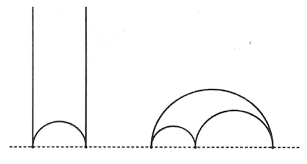
\includegraphics[width=.5\textwidth]{figures/hyperbolic_geometry.png}};
	\end{tikzpicture}
\end{figure}

We define a function $\phi : \mathbb H^2 \to \R / 2\pi\Z$ which to each pair $(p,q)$ of points in the Poincarè half-plane associates the angle between the vector $\vec{q\conj p}$ and the vector $\vec{q p}$ (in this order) or, equivalently, to the angle between the vertical line at $p$ and the geodesic between $p$ and $q$ (in this order):

\begin{figure}[H]
	\centering
	\begin{tikzpicture}
		\node (image) at (0,0) {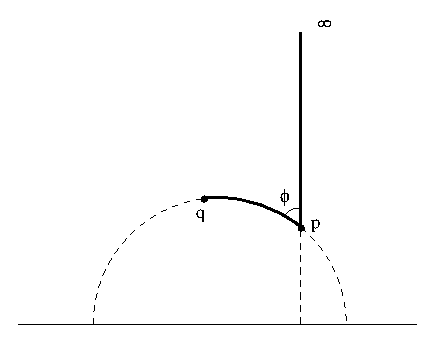
\includegraphics[width=.5\textwidth]{figures/kontsevich_graph_weight.eps}};
	\end{tikzpicture}
\end{figure}

Analytically, $\phi$ is given by
\begin{eqalign}
	(p,q) \longmapsto \arg\left( \frac{q-p}{q-\conj p} \right) = \frac{1}{2i} \log \left( \frac{q-p}{q \conj p} \cdot \frac{\conj q - p}{\conj q - \conj p} \right).
\end{eqalign}
This function is holomorphic over $\mathbb H^2$ and extends continuously to $\Im{p} = 0$ or $\Im{q} = 0$.

Now let $\Gamma \in G_n$ be an admissible graph. Let us denote with $R_n$ the set of possible isometrical embeddings of $\Gamma$ in $\mathbb H$ sending $L$ to $0$ and $R$ to $1$, i.e. the set of possible $n$-tuple of \underline{distinct} points from which we realize geometrically the graph $\Gamma$ using arcs of geodesics to draw the edges. Notice the set $R_n$ is actually independent of $\Gamma$, as any $n$-tuple of distinct points can be used to draw isometrically any graph in $G_n$.

\begin{figure}[H]
	\centering
	\begin{tikzpicture}
		\node (image) at (0,0) {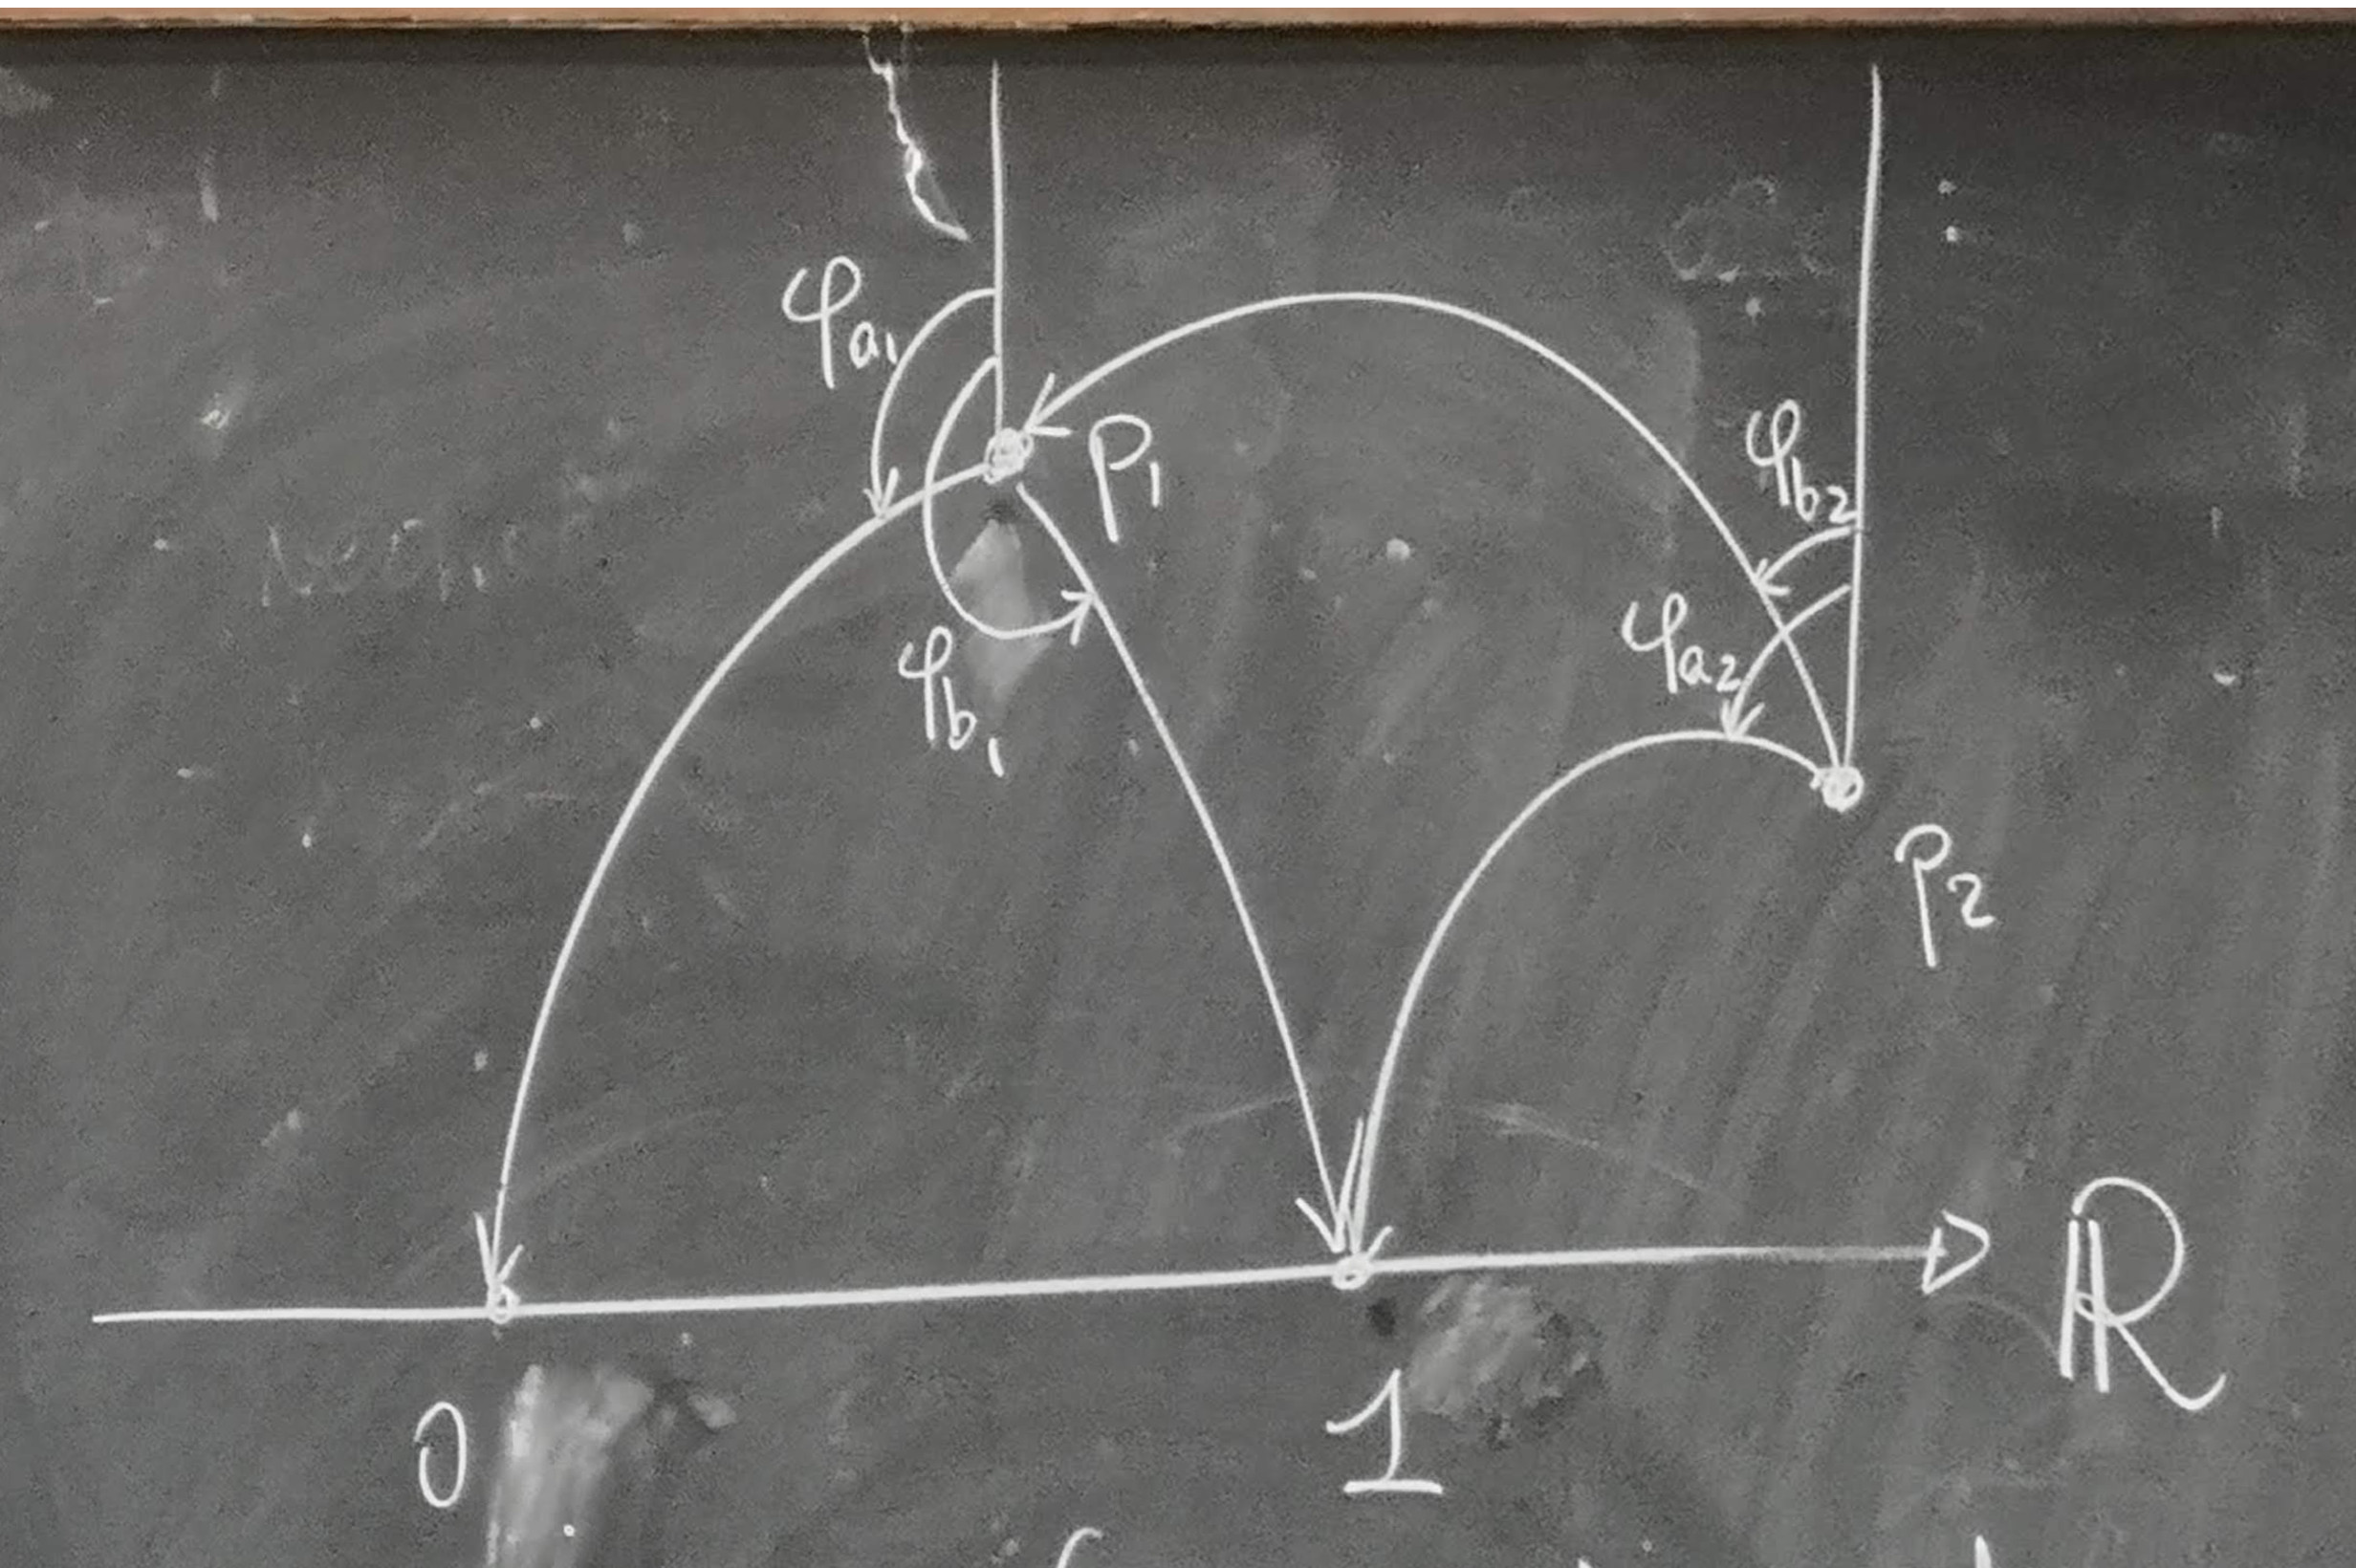
\includegraphics[width=.65\textwidth]{figures/may23_hyperbolic_immersion.jpg}};
	\end{tikzpicture}
	\caption{A realization of the admissible graph \eqref{diag:order_two_adm_graph}.}
	\label{fig:realization_ex}
\end{figure}

Given a realization $V_\Gamma \ni m \mapsto \overline{m} \in \mathbb H$, define $\phi_a$ to be $\phi(\overline{s(a)}, \overline{t(a)})$. Thus $\phi_a$ measure the abovementioned angle for the edge $a$. These are represented in Figure~\ref{fig:realization_ex}.

\begin{definition}
	The weight $w_\Gamma$ associated to $\Gamma \in G_n$ is defined as
	\begin{eqalign}
		w_\Gamma := \frac1{(2\pi)^{2n}} \int_{R_n} \bigwedge_{a \in E_\Gamma} d\phi_a.
	\end{eqalign}
\end{definition}

Then the integral can be done, with a change of variables, in the $\phi_{a_i}, \phi_{b_i}$ coordinates and it can be proven that

\begin{lemma}
	The integral defining $w_\Gamma$ converges absolutely for every admissible graph $\Gamma$.
\end{lemma}

\subsubsection{The formula}
Finally, we can write down the sought formula.

\begin{theorem}
	To a formal Poisson structure $\Pi_\planck$ it is associated the $\star$-product given by
	\begin{eqalign}
		f \star_\planck g := \sum_{n=0}^\infty \frac{\planck^n}{n!} \sum_{\Gamma \in G_n} w_\Gamma B_{\Gamma,\Pi_\planck}(f,g).
	\end{eqalign}
	Moreover, this definition is stable (up to equivalence of $\star$-products) under change of coordinates.
\end{theorem}

\begin{example}
	Let $\Pi_\planck = \Pi = \Pi^{ij} \partial_i \partial_j$, with $\partial_k \Pi^{ij} = 0$ for any $k$. This means that only those $\Gamma \in G_N$ with $t(E_\Gamma) \subseteq \{L,R\}$ contribute to the associated star product, as this guarantees no derivatives of the Poisson tensors appear in their term. Such graphs look like this:
	\begin{diagram}
	\label{diag:moyal_graphs}
		\& \Overset{1}\bullet \arrow{dl} \arrow{drrrr} \& \Overset{2}\bullet \arrow{dll} \arrow{drrr} \&[2ex] \dots \&[2ex] \Overset{n}\bullet \arrow{dllll} \arrow{dr}\\
		\Underset{L}\bullet \& \& \& \& \& \Underset{R}\bullet
	\end{diagram}
	where we didn't label the arrows as for each vertex there are two choices, so for each $n$ we get, in total, $2^n$ non-vanishing terms for the $n$th degree coefficient. The symmetry of exchanging $a_k$ with $b_k$ changes sign to $d\phi_{a_1} \wedge d \phi_{b_1} \wedge \ldots \wedge d\phi_{a_n} \wedge d\phi_{b_n}$, and so does $w_\Gamma$. On the other hand, the corresponding term also changes sign under this exchange, since a term $\Pi^{i_kj_k}$ changes to $\Pi^{j_ki_k} = - \Pi^{i_kj_k}$, by skew-symmetry. In the end, this gets us
	\begin{eqalign}
		B_n(f,g) = \frac1{n!} \sum_{\Gamma \in G_n} w_\Gamma B_{\Gamma, \Pi} = 2^n w_{\Gamma_n} B_{\Gamma_n,\Pi}
	\end{eqalign}
	where $\Gamma_n$ is the graph \eqref{diag:moyal_graphs} labelled as to have all $a_k$ edges going into $L$ and all the $b_k$ into $R$.

	We know what $B_{\Gamma_n, \Pi}$ looks like:
	\begin{eqalign}
		B_{\Gamma_n, \Pi} = \Pi^{i_1j_1} \cdot \ldots \cdot \Pi^{i_nj_n}\, \partial_{i_1}\ldots \partial_{i_n} f \, \partial_{j_1}\ldots \partial_{j_n} g.
	\end{eqalign}
	To compute the weight, we solve the relevant integral. Notice each vertex can be positioned in the same points (i.e. the condition $\overline{1} \neq \overline{2}$ is virtual), and that all angle variables relative to different vertices are independent as there are no edges between them. With these considerations, we can already simplify the computation to the following:
	\begin{eqalign}
		w_\Gamma = \frac1{(2\pi)^{2n}} \int_\hilbert d\phi_{a_1} \wedge d\phi_{b_1} \wedge \ldots \wedge d\phi_{a_n} \wedge d\phi_{b_b} = \frac1{(2\pi)^{2n}} \left( \int_\hilbert d\phi_{a_1} \wedge d\phi_{b_1} \right)^n.
	\end{eqalign}
	Then by fiddling around in the Poincarè upper half-plane, we see that (1) $\phi_a \leq \phi_b$ for any position and (2) all angles are achievable by a suitable configuration of the vertices. Therefore:
	\begin{eqalign}
	\frac1{(2\pi)^{2n}} \left( \int_\hilbert d\phi_{a_1} \wedge d\phi_{b_1} \right)^n = \left( \int_0^{2\pi} \int_0^{\phi_b} d\phi_a d\phi_b \right)^n = \frac1{(2\pi)^{2n}} \left(\frac{2\pi \times 2 \pi}2\right)^n = \frac1{2^n}.
	\end{eqalign}
	So, in the end we get the Moyal product:
	\begin{eqalign}
		f \star g = \frac1{n!} \Pi^{i_1j_1} \cdot \ldots \cdot \Pi^{i_nj_n}\, \partial_{i_1}\ldots \partial_{i_n} f \, \partial_{j_1}\ldots \partial_{j_n} g = f\, \exp\left( \Pi^{ij} \lpartial_i \rpartial_j \right)\, g = f \star_M g.
	\end{eqalign}
\end{example}

\begin{remark}
	The Moyal product is the $\star$-product associated to $\Pi = \Pi^{ij} \partial_i \wedge \partial_j$, where $\Pi^{ij}$ are constants. It's associated to the null deformation. Locally every constant rank Poisson tensor is expressible like that, in Darboux--Weinstein coordinates. This means that, locally, the first-order expansion of the associated product is:
	\begin{eqalign}
		f \star g = fg + \planck\, \Pi^{ij} \partial_i f\, \partial_j g + O(\planck^2).
	\end{eqalign}
\end{remark}

\section{Retrospect}
Our goal was to produce $(\Cinfty(M), \star)$ so as to have observables $f$ in there which obey the equation
\begin{eqalign}
	\partial_t f = \frac{i}\planck [f,h]_\star.
\end{eqalign}
In the undeformed setting, the evolution of $f$ was given by the time evolution operator (ref):
\begin{eqalign}
	f(t) = U(t)^\dagger \,f(0)\, U(t)
\end{eqalign}
In the deformed case we need to correct the operator, starting from the exponential:
\begin{eqalign}
	\exp_\star (g) = 1+g + \frac{g \star g}2 + \frac{g \star g \star g}6 + \ldots = \sum_{n=0}^\infty \frac{g^{\star n}}{n!}.
\end{eqalign}
To get predictions out of the theory, we need necessarily some states on which evaluate observables. Where do we get them? It turns out we can interpret some functions of the algebra as states (the so-called Wigner functions).
